% !TeX spellcheck = en_US
%\documentclass[12pt]{article}

\documentclass[11pt]{report}

\usepackage[a4paper, margin=1in]{geometry}

\usepackage{mathtools}
\usepackage{footnote}
\usepackage{listings}
\usepackage{xcolor}
\usepackage{mathtools}
\usepackage{pdfpages}
\usepackage[english]{babel}
\usepackage[labelfont=bf]{caption}
\usepackage{float}
\captionsetup{labelfont=bf}
\usepackage[normalem]{ulem}

\useunder{\uline}{\ul}{}

\definecolor{codegreen}{rgb}{0,0.6,0}
\definecolor{codegray}{rgb}{0.5,0.5,0.5}
\definecolor{codepurple}{rgb}{0.58,0,0.82}
\definecolor{backcolour}{rgb}{0.95,0.95,0.95}
\usepackage{titlesec, color}

\definecolor{gray75}{gray}{0.75}
\newcommand{\hsp}{\hspace{10pt}}
%\titleformat{\section}[hang]{\Huge\bfseries}{\thesection\hsp\textcolor{gray75}{|}\hsp}{0pt}{\Huge\bfseries}

\lstdefinestyle{mystyle}{
	backgroundcolor=\color{backcolour},   
	commentstyle=\color{codegreen},
	keywordstyle=\color{blue},
	numberstyle=\tiny\color{codegray},
	stringstyle=\color{orange},
	basicstyle=\ttfamily\footnotesize,
	breakatwhitespace=false,         
	breaklines=true,                 
	captionpos=b,                    
	keepspaces=true,                 
	numbers=left,                    
	numbersep=5pt,                  
	showspaces=false,                
	showstringspaces=false,
	showtabs=false,                  
	tabsize=2
}

\lstset{style=mystyle}

\includeonly{
	chapters/introduction,
	chapters/modeling,
	chapters/implementation,
	chapters/verification,
	chapters/simulation_experiments,
	chapters/conclusions
}

\begin{document}


\begin{titlepage}
	\begin{center}
		\begin{figure}
			
\includegraphics[width=\textwidth]{img/marchio_unipi_pant541-eps-converted-to.pdf}         
		\end{figure}
		{\Large
			Computer Engineering\\
			\vspace{5mm} %5mm vertical space
			Foundations of Cybersecurity}\\
		\vspace{30mm} %5mm vertical space
		{\Huge\textbf{\textit{secureCom}}}\\
		\vspace{10mm} %5mm vertical space
		{\Large Group Project Report}\\
		\par\noindent\rule{\textwidth}{0.4pt}
		\begin{flushright}
			\textit{TEAM MEMBERS}:\\ 
			Francesco Iemma\\
			Yuri Mazzuoli\\ 
			Olgerti Xhanej\\
			
		\end{flushright}
		\vfill
		Academic Year: 2020/2021\\        
	\end{center}
\end{titlepage} 
\tableofcontents
\chapter{Specifications}
	\noindent The project consists on an application for secure communication between 2 clients through an intermediate server.
	\newline
	The server has to:
	\begin{itemize}
		\item authenticate clients when they connect to the server (with pre-shared public key)
		\item authenticate itself with a certificate
		\item provide the list of online clients
		\item relay messages from one client to another, together with chat requests and response
		\item provide to a client the public key of another client, in order to permit a secure communication between them
	\end{itemize}
	A client has to:
	\begin{itemize}
		\item authenticate the server (with the certificate)
		\item authenticate himself with its public key
	\end{itemize}
	A client can:
	\begin{itemize}
		\item print the list of online clients
		\item authenticate another client via its public key obtained from the server
		\item request to chat with another client
		\item answer to a chat request (if not already involved in another chat)
		\item when in a chat, exchange text messages with another client or close the chat
	\end{itemize}

\newpage
\chapter{Design choices}
\section{Client Server Handshake}
In order to authenticate themselves and establish a session key to securely communicate, a client
and the server have to exchange handshake messages. We implement this protocol to provide perfect 
forward secrecy, starting from the pre-shared cryptographic quantities (public keys and certificates):

\begin{figure}[H]
	\centering
	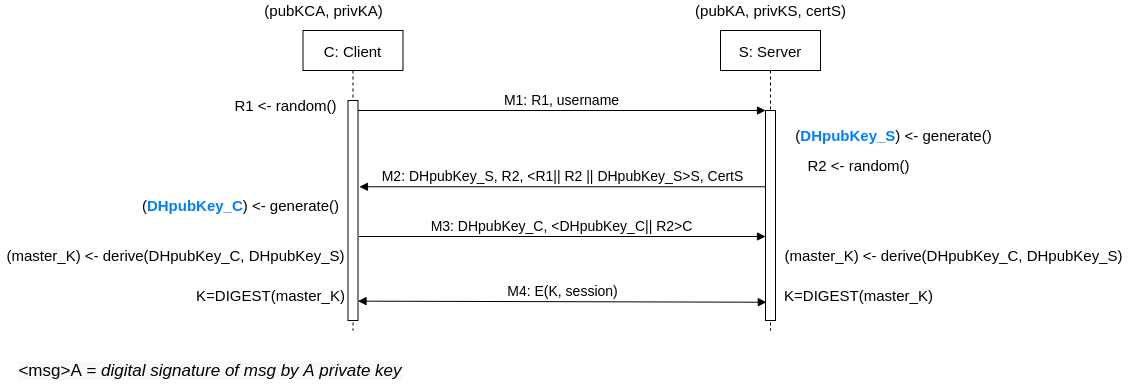
\includegraphics[scale=0.2]{img/AuthClientServer.png}
	\caption{Client Server Handshake Protocol Schema}
	\label {img: AuthClientServer}
\end{figure}

\noindent This handshake is a custom implementation of an ephemeral Diffie-Hellman Key Exchange, in which we ensure
protection against the man in the middle attack with random nuances (R1 and R2). The client is able to 
authenticate the server via it's certificate, signed by a trusted certification authority (the client
is distributed along with CA's self-signed certificate); the server has a built-in list of all client's
public keys. DH's private keys are deleted after the handshake and the session key is generated by a digest of the 
shared secret: in this way we provide security against a possible future disclosure of one of the long term private keys.

\newpage
\section{Chat Request}
With the client-server handshake we build a secure tunnel between each client and the server. Using this 
tunnel every client can execute command on the server in a secure way; the most important (and complex) command
is a chat request, of which we provide a scheme:
\begin{figure}[H]
	\centering
	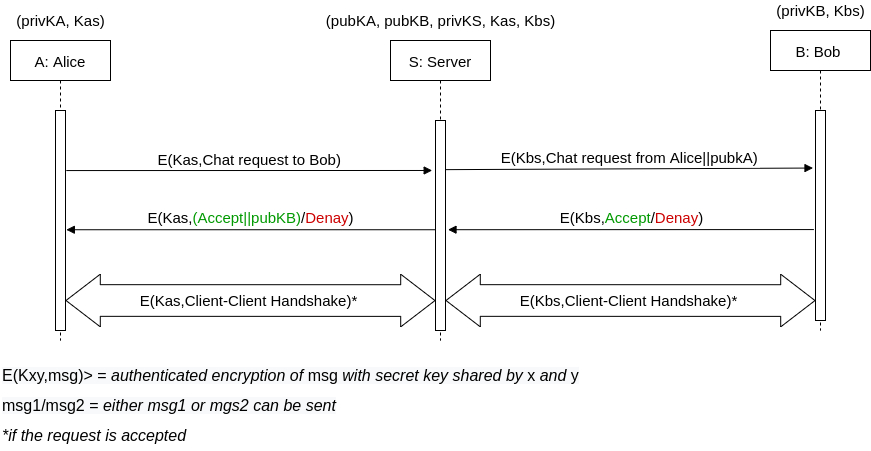
\includegraphics[scale=0.2]{img/ChatRequest.png}
	\caption{Chat Request Protocol Schema}
	\label {img: ChatRequest}
\end{figure}
\noindent In this case the security is based on the assumption that the server is obliged to communicate correct public keys. This assumption is fulfilled since the server is considered honest-but-curious.

\section{Client to Client handshake}
In order to guarantee a secure communication of the clients against the server, we perform an ephemeral 
Diffie-Hellman Key Exchange before starting the chat. In this case the two parties already know each other
public keys, because the server provided them. 

\begin{figure}[H]
	\centering
	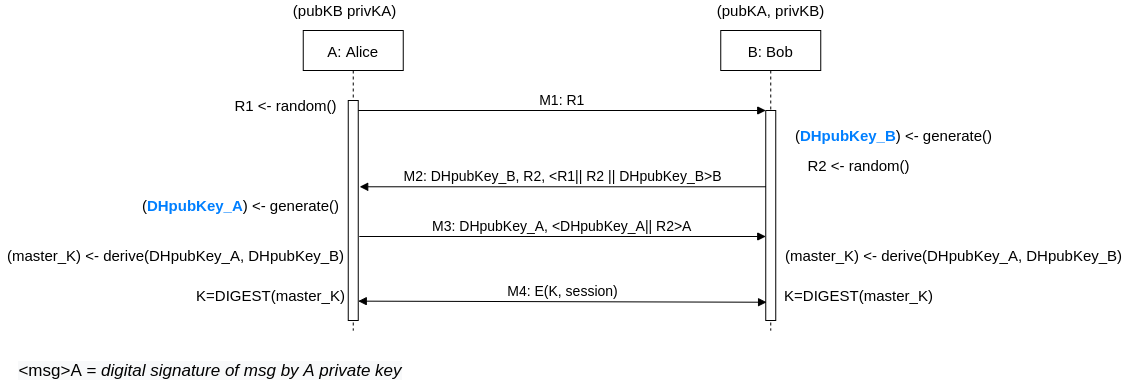
\includegraphics[scale=0.19]{img/AuthClientClient.png}
	\caption{Client Client Handshake Protocol Schema}
	\label {img: AuthClientClient}
\end{figure}

\noindent The server in not represented because it only re-transmit messages from a client to the other without changing
anything; if the server try to implement a "man in the middle" attack he will only obtain a denial of service
because the protocol is protected by private key signatures. Also in this case, DH keys are discarded after 
the handshake, and future messages are numbered against reply attacks.

\section{Session Ending}
In order to end a chat session, one of the two users may send a \texttt{STOP CHAT} command to the server; this
command is forwarded to the other client, who will close the chat session by his side; in order to disconnect from the server, the user have to send the 
\texttt{EXIT} command. In case one client stops without sending the \texttt{EXIT} command, the server will notice 
it and will proceed to close the session and (if necessary) relative chat session.


\chapter{Implementation}
\section{Software Architecture}
From an implementation viewpoint, the client program has to communicate with the user and the server; in the
server program instead, messages have to pass from one process to another in order to be delivered to the
recipient client. In the figure \ref{img: Implementation_scheme} we can see the implementation scheme.

\begin{figure}[H]
	\centering
	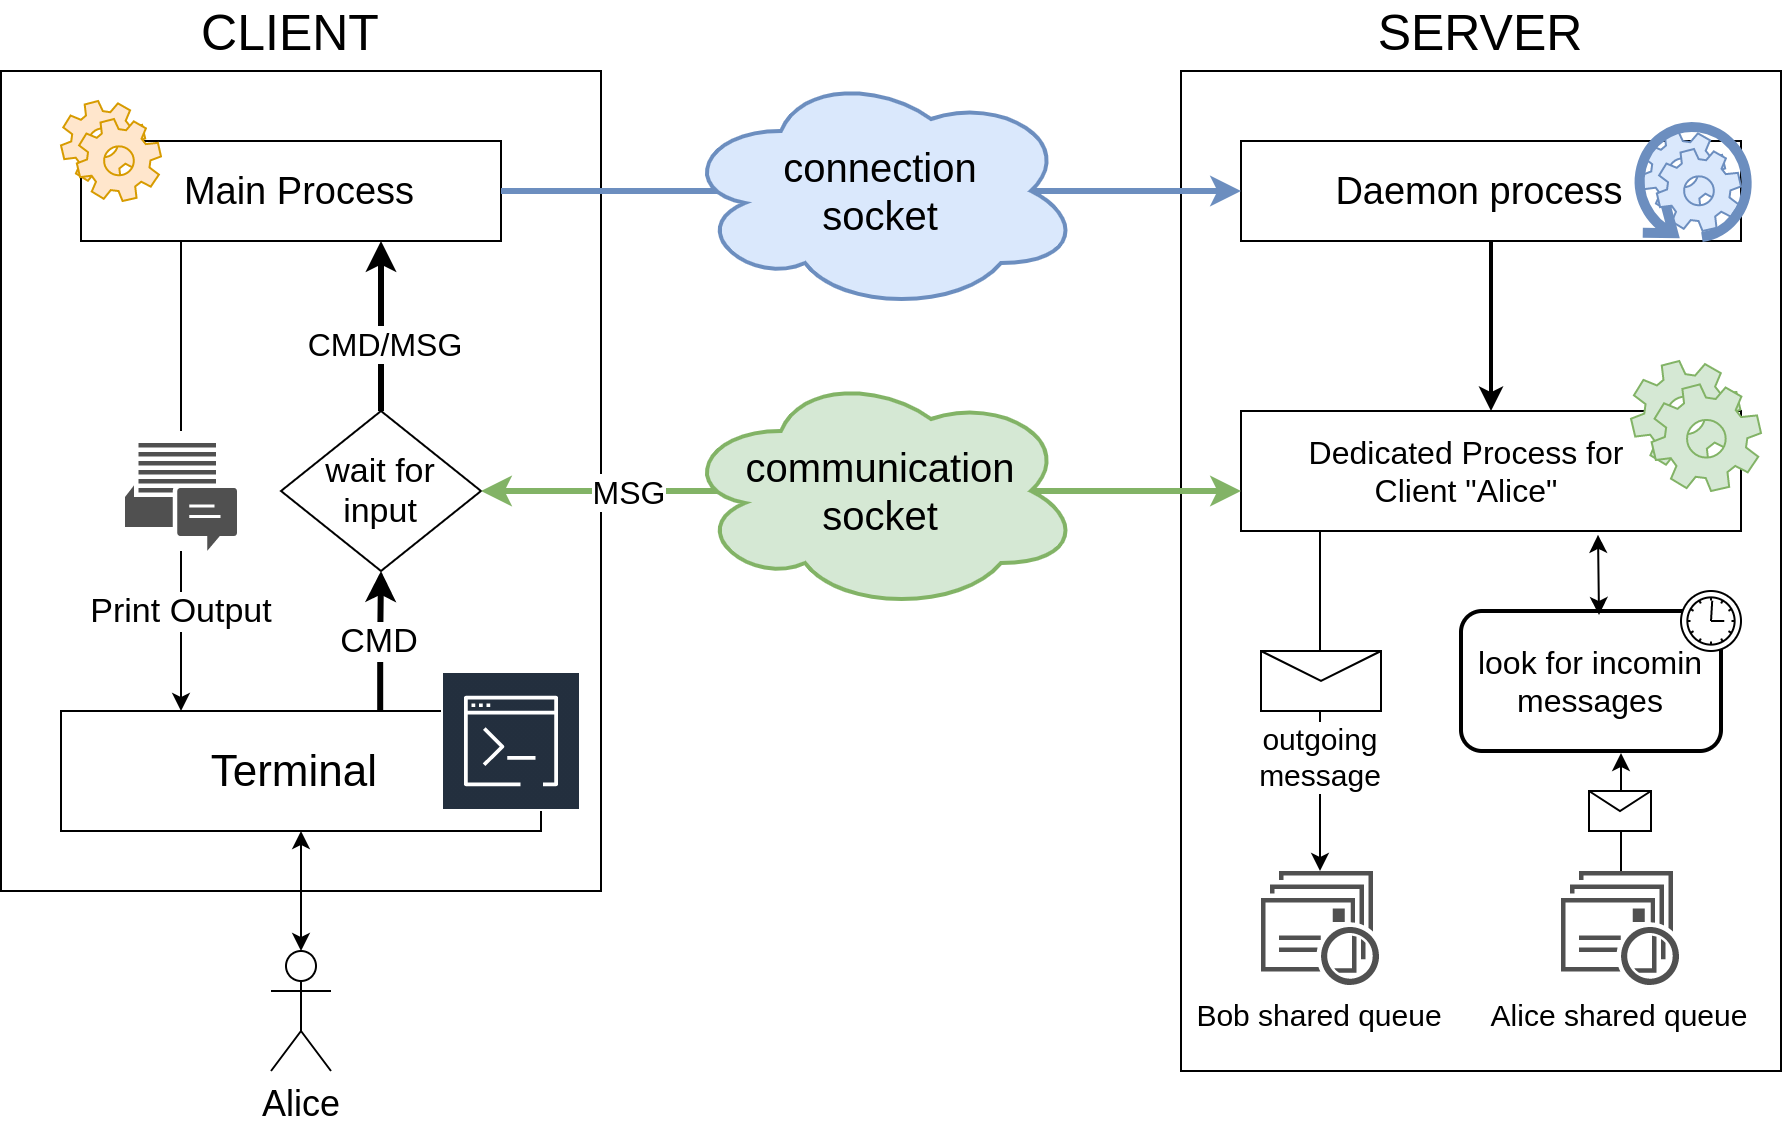
\includegraphics[scale=0.24]{img/Implementation_scheme.png}
	\caption{Implementation scheme}
	\label {img: Implementation_scheme}
\end{figure}

\noindent At the beginning the client will connect to a standard server port which is in listening state; then the communication
is commuted to another port, with a dedicated server process. At the end of the secure handshake, the process will be 
dedicated to the authenticated user who is connected. This server process is able to read from his dedicated queue of 
incoming messages, and relay messages to others client via their queue; at constant intervals a timer will read all the 
messages from the incoming queue and it will forward them to the client. When this behavior is unwanted, the relative interrupt
is disabled.


\noindent Using the system call \texttt{select()} the client is able to listen from multiple sources of input, in this
case the sources are: communication socket and terminal. In this way the client program is able, for example, to automatically refuse a chat request 
when the user is already chatting or it is in the authentication phase with another client.

\section{Algorithms and Protocols}
We briefly describe the cipher suite we choose to use in order to guarantee security requirements.
Ciphers are the same for Client-Server and Client-Client communication, specific message formats are reported In
Chapter 4.
\subsection{Public Key Authentication}
\paragraph*{Long Term Keys}
The Certification Authority (CA) has a \texttt{Public Key}, included in a self-signed
certificate; the corresponding private key is embedded in the program for certificate generation, 
SimpleAuthority \footnote{https://simpleauthority.com}.
CA's certificates and Revocation List (CRL) are exported and distributed with client executable.
The server certificate, which is signed by CA, contains the \texttt{Public Key} of the server; it
is stored server side, and provided to the client during the handshake.
Clients Public Keys are also stored in the server, while only the client hold its Private Key.
All keys are \texttt{RSA Key Pairs with 2048-bits Public Keys} and are stored in \texttt{.pem} format, as certificates and CRLs are.
\paragraph*{Short Term Keys}
Handshakes protocols are performed with the Ephemeral Diffie-Hellman Key Exchange. 
We choose to use the Elliptic Curve implementation because is very efficient (in term of performance vs security strength);
we use \verb|NID_X9_62_prime256v1| standard parameters that ensure 128-bits security strength with a 256-bits curve. We use the \texttt{SHA-256} digest of the \texttt{shared secret} as
the session key.
To ensure freshness in the challenge-response scheme we use \texttt{2 bytes nonces}.
\subsection{Authenticated Encryption}
From the handshake we obtain a 256-bits symmetric key which is used in \texttt{AES-256 GCM} authenticated encryption protocol.
We use a \texttt{16 bytes} tag for authentication of ciphertext and clear fields in the header. GCM scheme ensure a ciphertext
size equal to the plaintext size; this makes programming easier, maintaining an optimal resistance against all known attacks.
Messages exchanged in sessions are numbered, starting from 1, to a maximum of $2^{32}-1$ (\verb|0xFFFFFFFF|), which is the
maximum integer representable on 32 bits; this will make possible to identify a message reply, done
by an attacker. The session is automatically closed when a message with number \verb|0xFFFFFFFF| is received.
Clients maintains two counter for the communication with the server:  one for the next message to send and another for
the next message to receive; the same thing is done for the communication with another client (to prevent the server to 
reply a message); also the server has to implement this behavior in sessions with clients.

\subsection*{Note on Chat message encryption }
Chat message are encrypted twice, one time with the Client-Client session key and 
the second one with Client-Server session key; this will not double the BIT strength of the cipher against 
a brute force attack, because of the \texttt{meet in the middle} attack. 
At the same time, this fact makes the system more secure against a password recover attack; in case, for
whatever reason, a session key between clients is discovered by an attacker, this will not be enough for read private messages,
because the attacker have to discover also the session key between a client and the server.

\chapter{Messages Format}

\section{Handshake}
\subsection*{Client Server Handshake}
\begin{figure}[H]
	\centering
	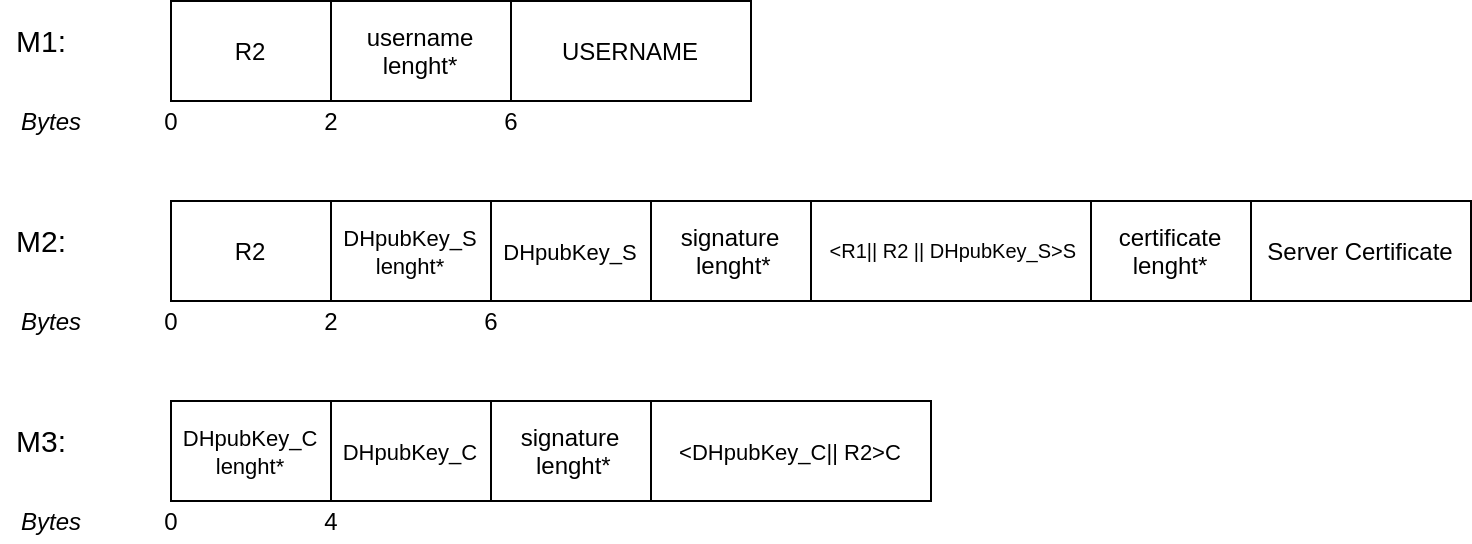
\includegraphics[scale=0.28]{img/AuthClientServer_messageFormat.png}
	\caption{Client Server Handshake Message Format}
	\label {img: FormatClientServer}
\end{figure}
\subsection*{Headers}
\begin{figure}[H]
	\centering
	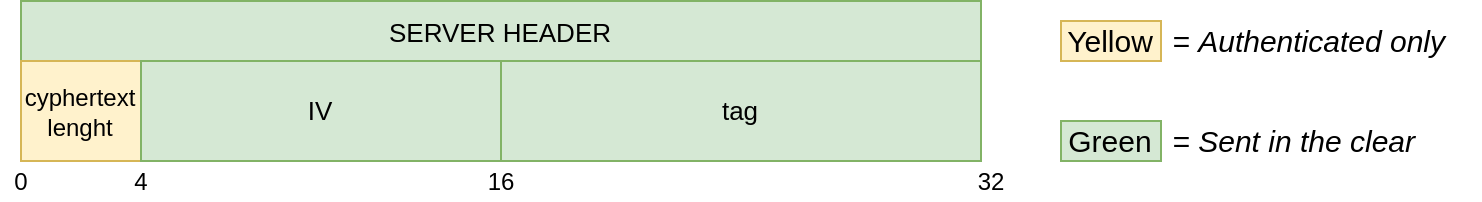
\includegraphics[scale=0.24]{img/HeaderFormat.png}
	\caption{Client Server Header Format}
	\label {img: FormatClientServerHeader}
\end{figure}
\subsection*{Client Client Handshake}
\begin{figure}[H]
	\centering
	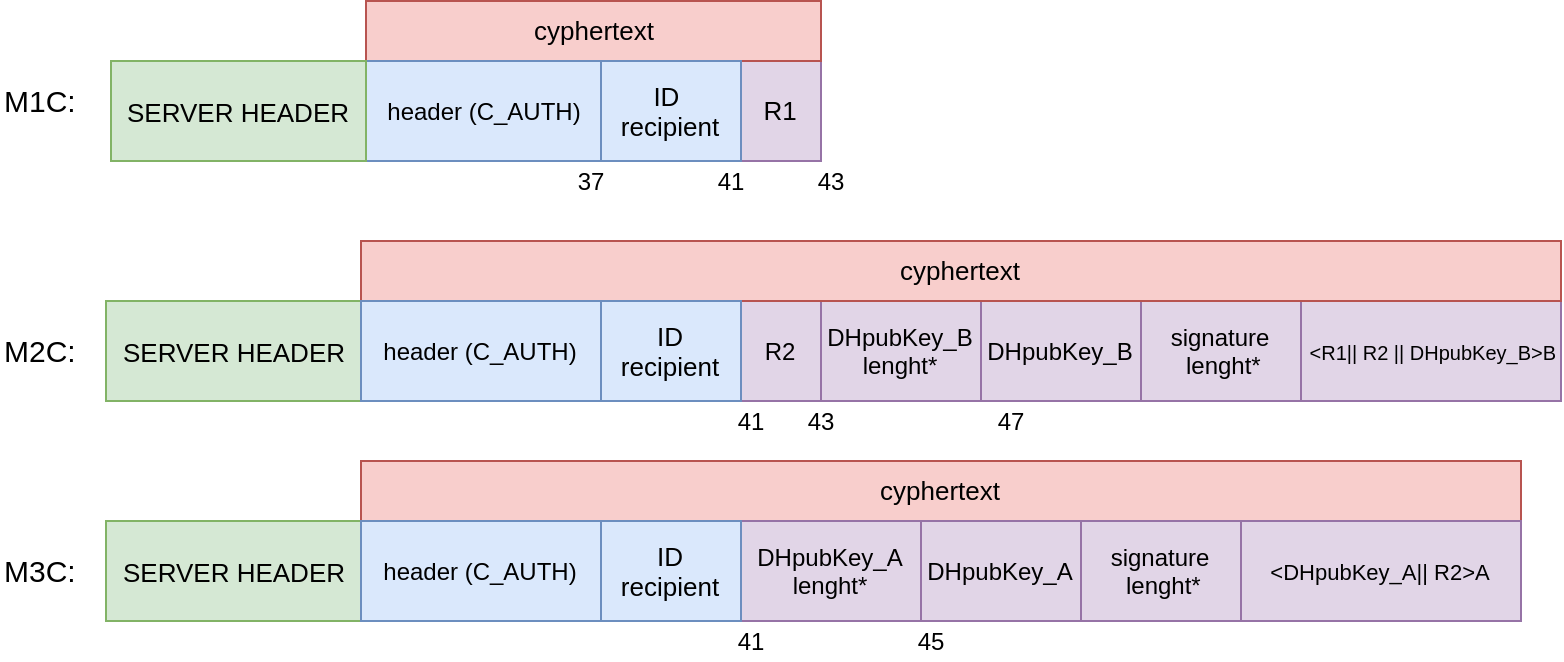
\includegraphics[scale=0.28]{img/AuthClientClient_messageFormat.png}
	\caption{Client Client Handshake Message Format}
	\label {img: FormatClientClient}
\end{figure}

\section{Commands}
\begin{figure}[H]
	\centering
	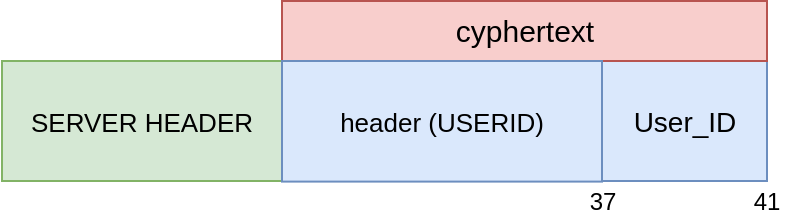
\includegraphics[scale=0.28]{img/SessionFirstMessageFormat.png}
	\caption{First message of every Session: server communicate client userID}
	\label {img: FormatClientServerFirst}
\end{figure}
\subsection*{Client Online List Request and Answer }
\begin{figure}[H]
	\centering
	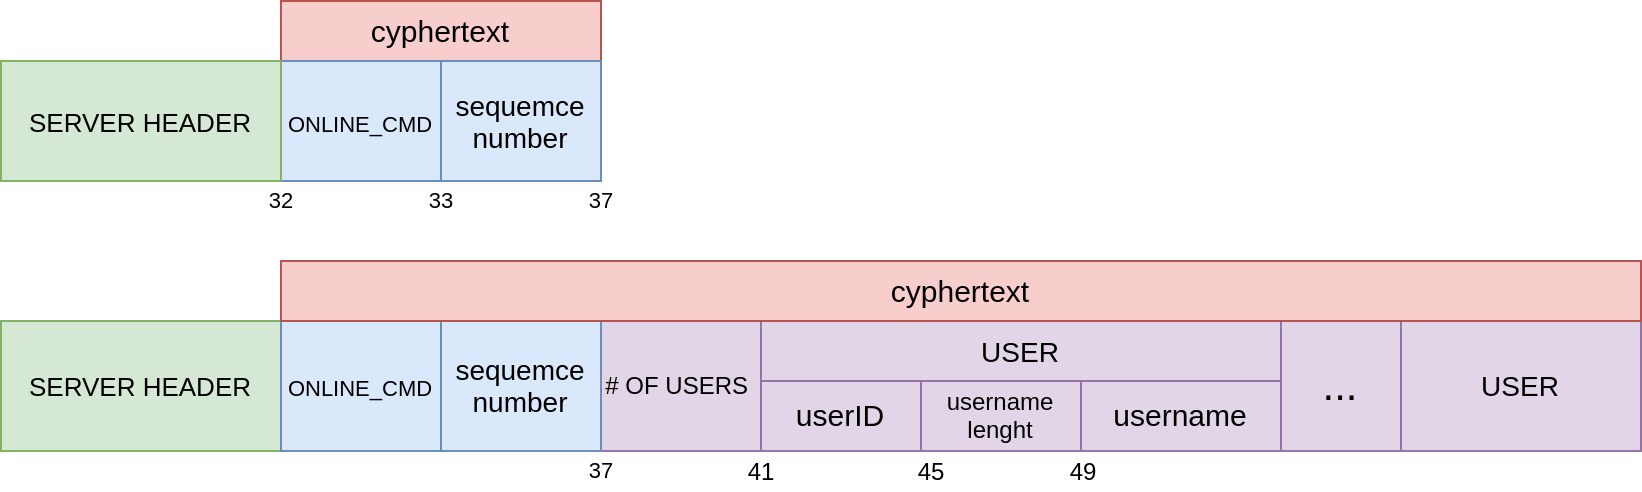
\includegraphics[scale=0.25]{img/ClientOnline_messageFormat.png}
	\caption{Client Online Message Format}
	\label {img: FormatClientOnline}
\end{figure}
\subsection*{Other commands}
\begin{figure}[H]
	\centering
	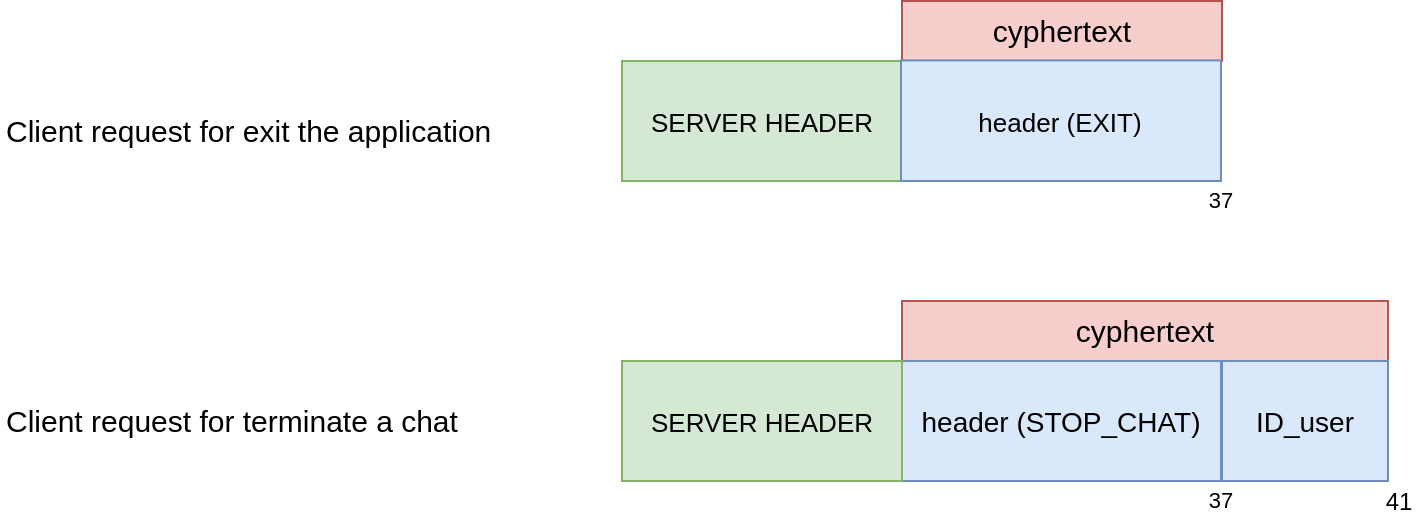
\includegraphics[scale=0.28]{img/OthersCommandsFormat.png}
	\caption{Other commands Format}
	\label {img: FormatOtherCommands}
\end{figure}
\subsection*{Chat Request and Answers}
\begin{figure}[H]
	\centering
	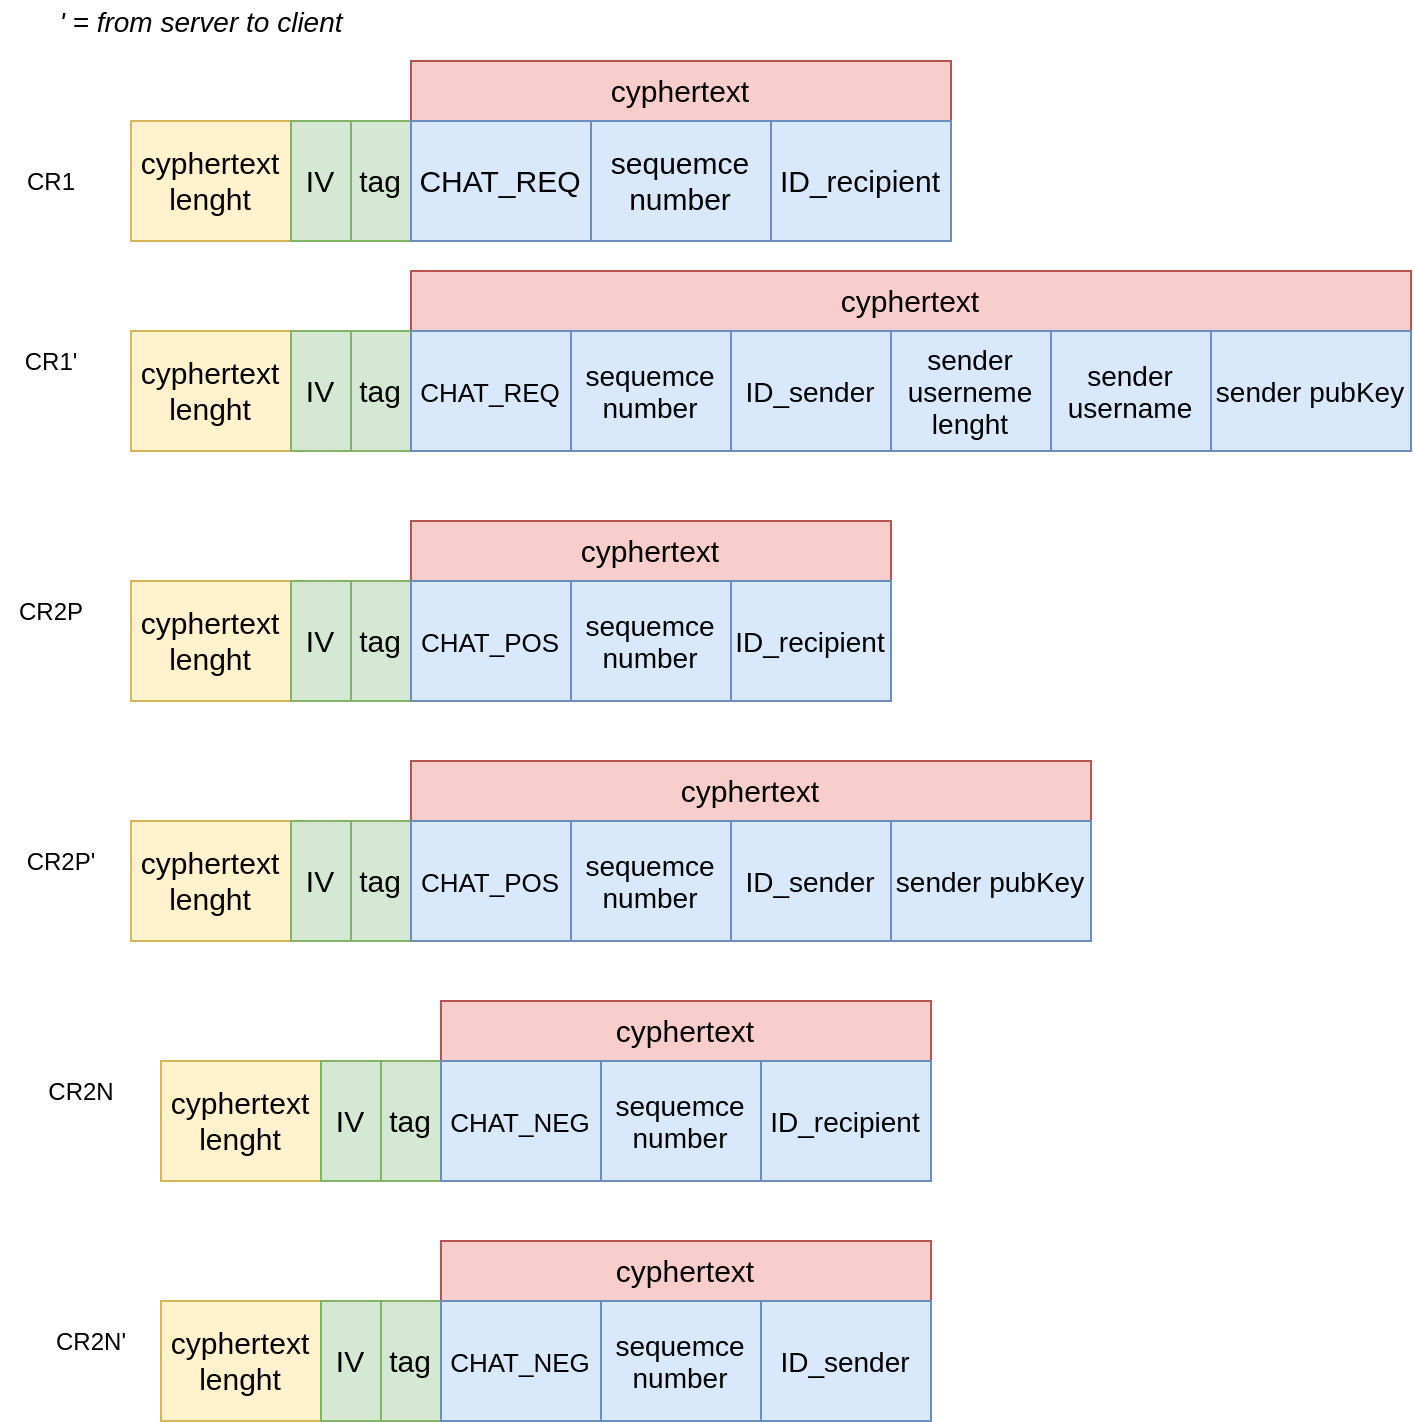
\includegraphics[scale=0.28]{img/ChatRequest_messageFormat.png}
	\caption{Chat Request Message Format}
	\label {img: FormatChatRequest}
\end{figure}
\newpage

\section{Chat}
\begin{figure}[H]
	\centering
	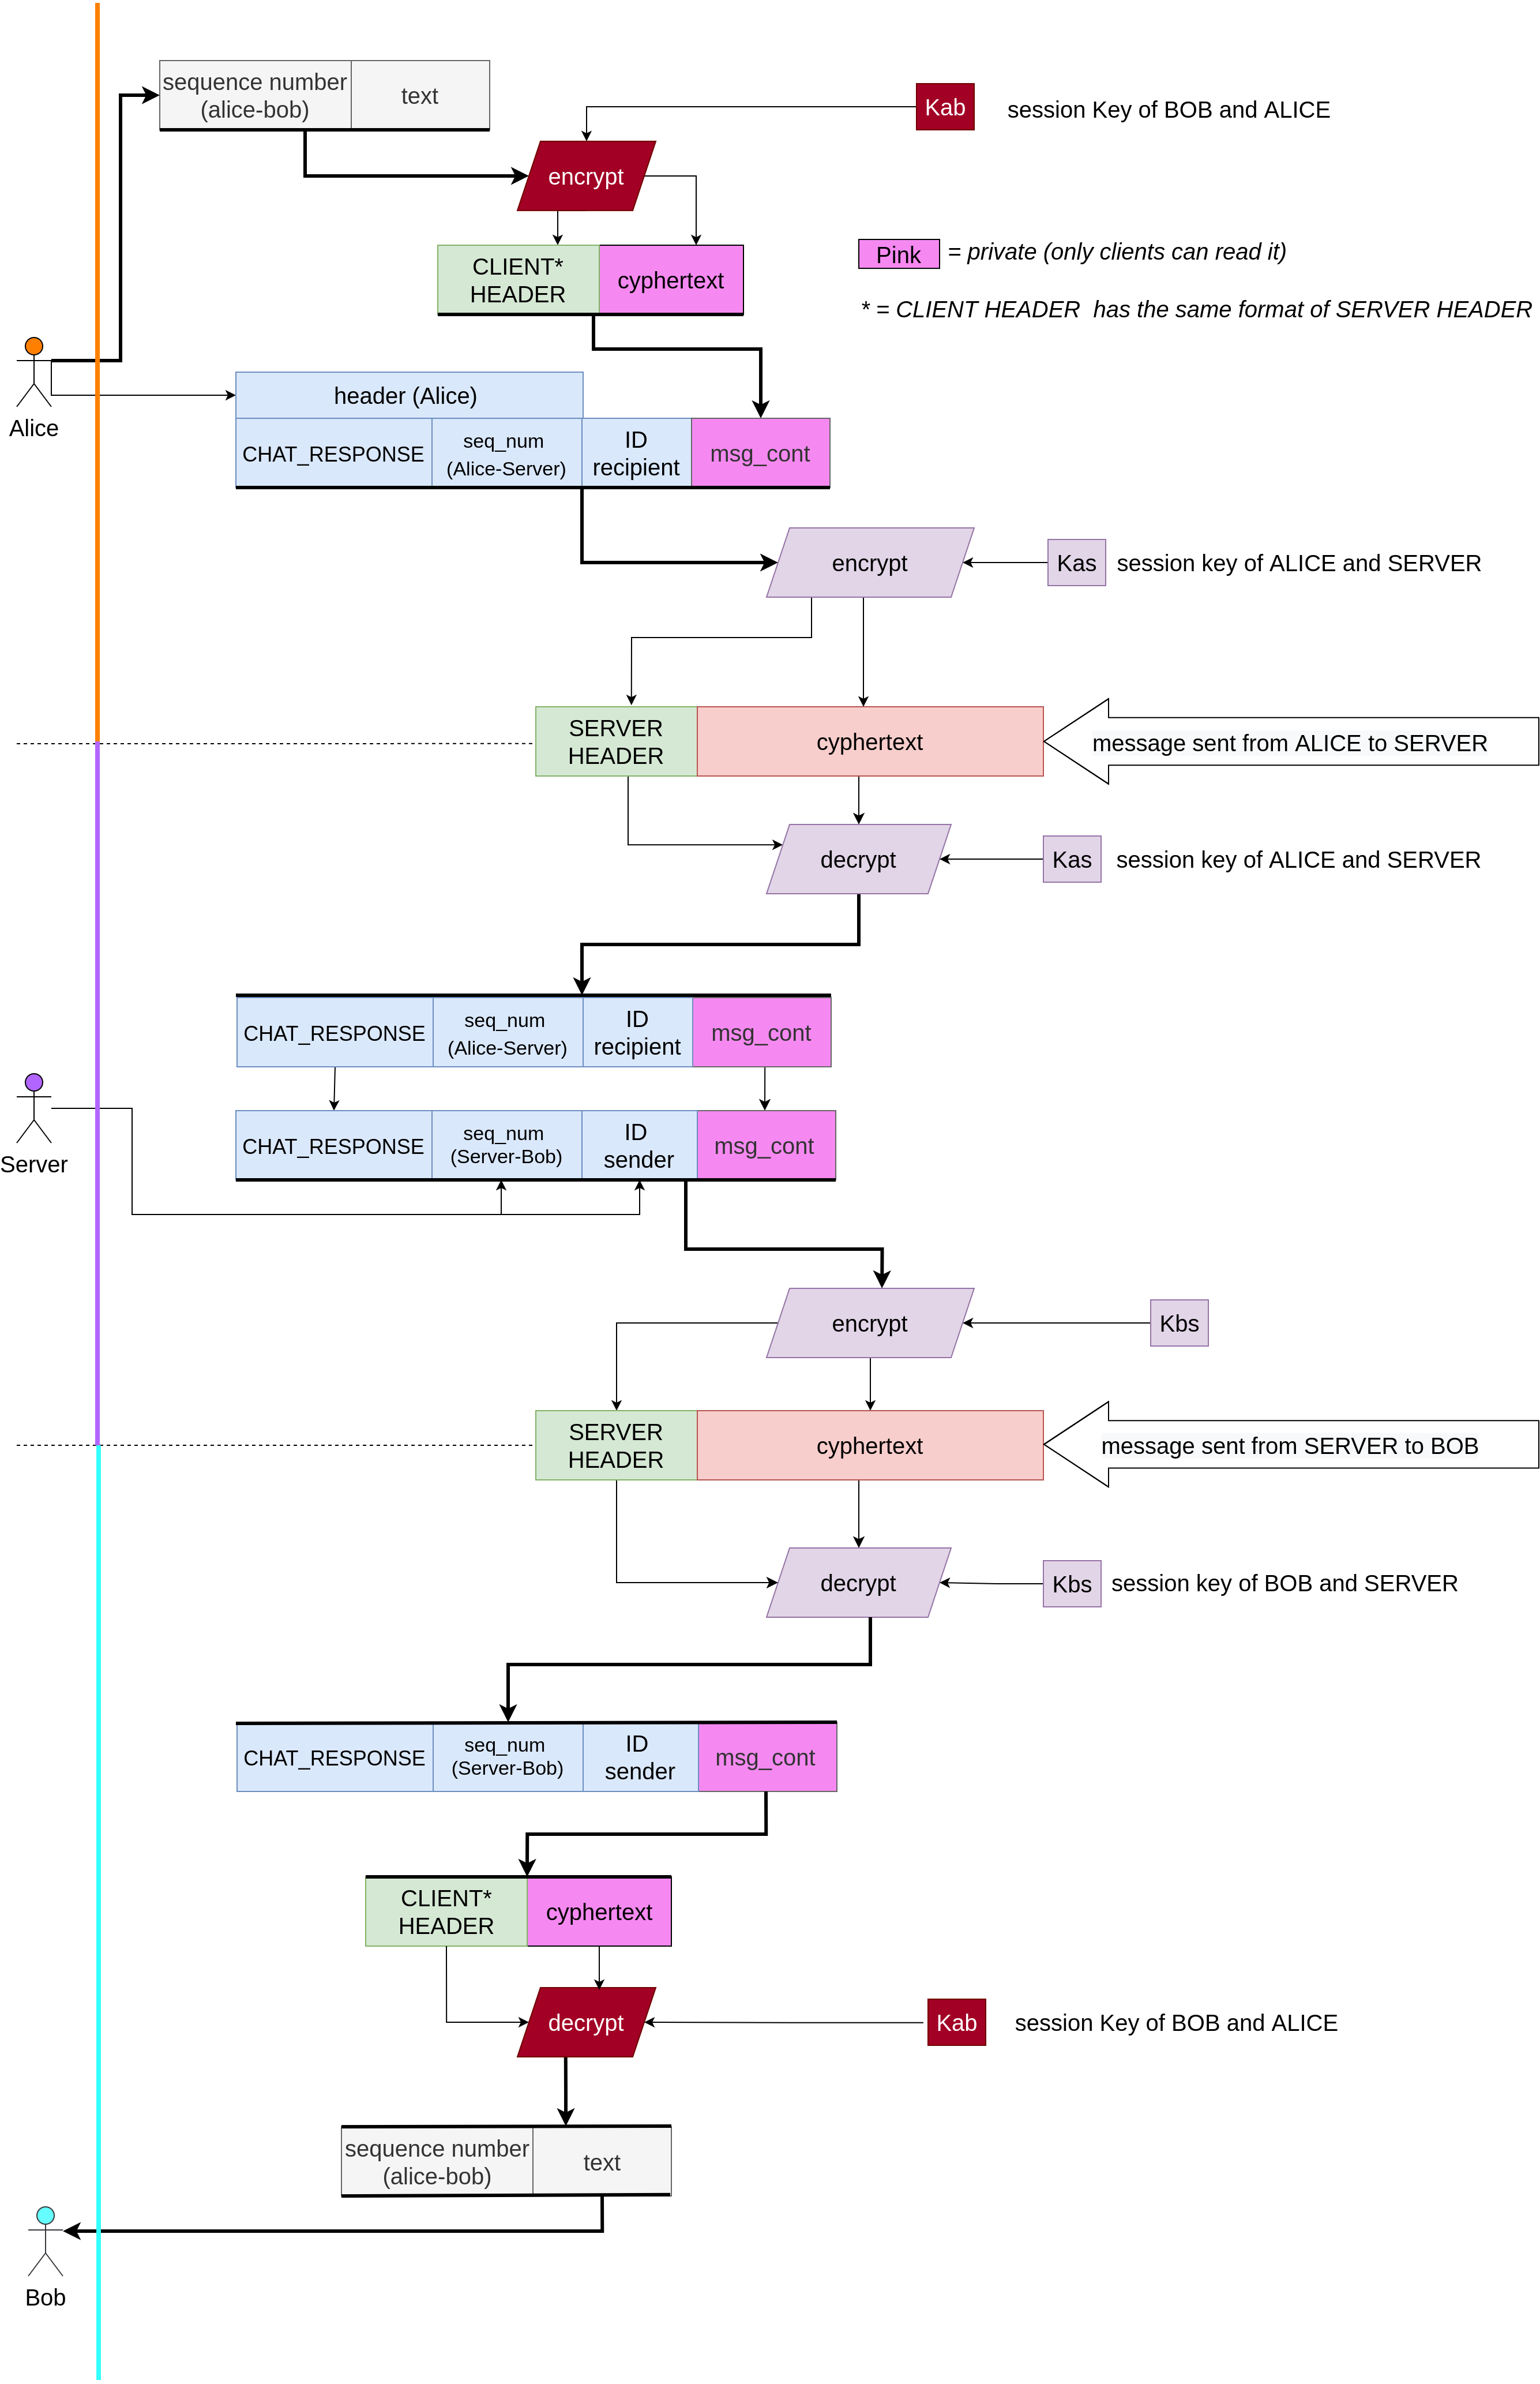
\includegraphics[scale=0.15]{img/message_relay.png}
	\caption{Client Client Handshake Protocol Schema}
	\label {img: MessageRelay}
\end{figure}


\chapter{User Manual}
\subsection*{Server}
The server is a daemon, so it has to be started and it will be always running. At server startup a password
a \texttt{sudo} password is required in order to properly set kernel variables for the message queue; than another password
is required, this time to decrypt and use the private key, which is stored in the \verb|SecureCom_prvkey.pem| file.

\section{Login}
At client startup the user need to insert his/her username and the password to decrypt and use his private key:
\begin{lstlisting}
*********************************************************************** 
                        SECURE COMMUNICATION 
*********************************************************************** 
!exit       Close the application
!help       See all the possible commands
-------------------------------------------------------------------------
Who are you? 
> alice
Enter PEM pass phrase:
--- AUTHENTICATION DONE --- 
HELLO alice
\end{lstlisting}
At the end of this phase client and server have correctly authenticated each others and can now communicate
using a session key.
\newpage
\section{Chat}
\subsection*{Users list}
With this command a client can retrieve the list of online users:
\begin{lstlisting}
!users_online

**** USER LIST **** 
	ID 	 Username
	0 	 alice
	1 	 bob
****************** 
\end{lstlisting}

\subsection*{Chat request}
With the chat command, a client can request to chat with another one who is online:
\begin{lstlisting}
!chat
	
******************************************************
Write the userID of the user that you want to contact
> 0
Wait for user's response and authentication ....
Enter PEM pass phrase:
AUTHENTICATION WITH alice SUCCESFULLY EXECUTED 
\end{lstlisting}
\subsection*{Chat response}
when a chat requests is received, the user is asked to accept ot deny it; in case of positive answer,
handshake is performed (password is required at both sides).
\begin{lstlisting}
**********************************************************
Do you want to chat with bob with user id 1 ? (y/n)
y
Wait for authentication ... 
Enter PEM pass phrase:
Wait ...
AUTHENTICATION WITH bob SUCCESFULLY EXECUTED 
\end{lstlisting}
\newpage
\subsection*{Messages}
In the chat, text messages can be sent and received; received messages are printed on the right.
\begin{lstlisting}
++++++++++++++++++++++++++++++++++++++++++++++++++++++++++++++++++++
                            CHAT                                   
All the commands are ignored in this section except for !stop_chat 
Send a message to bob
++++++++++++++++++++++++++++++++++++++++++++++++++++++++++++++++++++ 

this is a secure message
                                    bob -> also this
!stop_chat			
                    +++ Chat terminated +++
\end{lstlisting}

	
%	\item A third solution can be adding a command to indicate that a client is available to receive chat request. Thus:
	
%	\begin{enumerate}
%		\item A users is online when it has launched the command "available" (isChatting = false). Notice that in this case the variable isChatting can be called in a more correct way isAvailable.
		
%		\item  A users is offline (isChatting = false) if it is not available (if he has not launched the command available or if he is chatting with someone else). In that case offline means also busy whereas online means also available.
%	\end{enumerate}

	
%\end{enumerate}

%here are two possibilities:
%\begin{enumerate}
%	\item Two processes, one for the client main process and another one for the client daemon process. See figure \ref{img: chatRequestProtocolTwoProcesses}.
	
%	\begin{figure}[htpb]
%		\centering
%		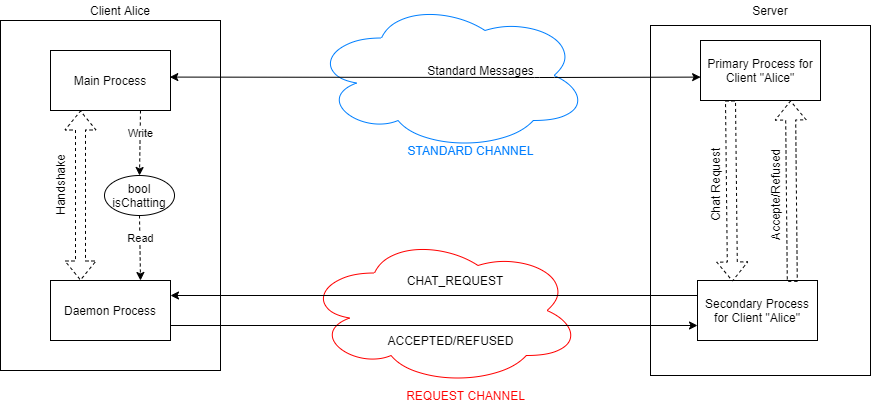
\includegraphics[scale=0.5]{img/chatRequestProtocolTwoProcesses.png}
%		\caption{Solution with two processes}
%		\label {img: chatRequestProtocolTwoProcesses}
%	\end{figure}

%\noindent Notes:


\end{document}          
